\chapter{Форирование ключевых подходов к CI/CD и проектирование доменной модели} \label{ch:ch2}

\section{Анализ и кластеризация репозиториев к переносу} \label{sec:repository-analysis}
Для стандартизации пайплайнов и оптимизации работы через GitLab API был получен список репозиториев компании.
Далее был написан скрипт,
который на основе названия репозитория (часть имела префикс, указывавший на тип репозитория) и использовавшихся в немы компонентов в GitHub Action,
определял, к какой категории данный репозиторий принадлежит.
Для репозиториев, у которых не получилось автоматически определить их тип, анализ выполнялся вручную.
По результатам анализа удалось выделить 26 кластеров, далее описаны некоторые из них:
\begin{itemize}
  \item Custom — репозиторий с уникальными пайплайнами, требующие отдельного подхода к переносу.
        В основном в эту категорию попадали старые большие проекты компании;
  \item CSharpLib — C\# библиотека со стандартизованными пайплайнами;
  \item CSharpLibNotTemplate — C\# библиотека с не стандартизованными пайплайнами;
  \item Microservice — C\# микросервис, использующий стандартизованные пайплайны;
  \item MicroFrontend — микрофронтенд;
  \item CopyOnly — репозиторий без CI/CD шаблонов, который можно просто скопировать;
  \item GitLeaksOnly — репозиторий, содержащий только стандартизированный gitleaks пайплайн.
\end{itemize}

\section{Выявление ключевых различий между GitHub Actions и GitLab CI/CD} \label{sec:gh-and-gl-differences}
Помимо типов репозиториев перед миграцией также были выявлены три основных области, где подходы GitHub Actions и GitLab CI/CD существенно отличаются друг от друга.
Каждое из этих различий требует специфических решений и обходных путей для обеспечения функциональной эквивалентности переносимых конвейеров.
\begin{itemize}
  \item Запуск процессов CI/CD по расписанию в формате cron.
        В GitHub подобный запуск описывается в конфигурации конвейера,
        а в GitLab необходимо настраивать расписание либо через сетевые запросы к сервису,
        либо через пользовательский интерфейс.
  \item Матрицы позволяют запускать несколько аналогичных конвейеров с разными параметрами.
        В GitLab CI/CD отсутствует возможность создания динамических матриц, поддерживаются только статические.
        Однако для данной проблемы было найдено обходное решение, которое будет описано далее.
  \item Шаги с выполнением кода или вызовом действий (actions).
        В GitHub Actions шаги могут либо выполнять определенный код, либо вызывать отдельное, заранее написанное действие.
        Все шаги выполняются в одном контексте, что позволяет использовать результаты предыдущих шагов в текущих.
        Это упрощает многие сценарии, например, сборку проекта или образа с последующей загрузкой результата на удаленный сервер.
        В GitLab недавно появился аналог этой функциональности, но он пока недостаточно развит.
        Его ограничения, как и в случае с динамическими матрицами, будут рассмотрены далее.
\end{itemize}

\section{Формирование ключевых подходов создания конвейеров} \label{sec:gitlab-pipelines-key-principles}
\subsection{Недостатки шагов в GitLab} \label{subsec:gitlab-steps-problems}
Основным фундаментальным отличием процессов конвейеров GitHub от GitLab является использование шагов вместо задач (jobs).
Задачи, в отличие от шагов, не сохраняют контекст выполнения, что в некоторых ситуациях требует его передачи между задачами,
что замедляет конвейер из-за дополнительных сетевых взаимодействий.
Поэтому структуру шагов хотелось бы сохранить.
В GitLab, как ранее было сказано, появился их аналог.
Однако на данный момент он является экспериментальным и имеет ряд проблем:
\begin{itemize}
  \item Это нововведение находится на стадии разработки, и некоторые параметры могут существенно измениться.
        В нашем случае это требует заморозки текущей версии исполнителя шагов, чтобы избежать неожиданных поломок.
        Однако при обновлении версии могут возникнуть ломающие изменения, что потребует значительной переработки кода;
  \item Не поддерживается условное выполнение шага.
        Шаг запустится, даже если предыдущие шаги завершились с ошибкой.
        Чтобы избежать этого, необходимо явно прописывать условия в коде шага, что непрактично для общих шагов, используемых в нескольких репозиториях.
        Было найдено решение в виде промежуточного шага, который принимает на вход данные о шаге, условие запуска и с помощью образа исполнителя шагов рекурсивно запускает или пропускает нужный шаг.
        Однако из-за рекурсивности это решение значительно замедляет работу при большом количестве вложенных условий;
  \item Отсутствие выражений, аналогичных GitHub, для написания базовых условных конструкций, включая методы, такие как поиск элемента в массиве.
        Это приводит к тому, что, даже если шаг успешно выполнился, необходимо вручную проверять условия внутри самого шага, что непрактично для переиспользуемых действий;
  \item Невозможно разрешить определенному шагу завершиться с ошибкой без остановки всего конвейера.
\end{itemize}

В связи с этими проблемами было решено отказаться от использования шагов в GitLab.

\subsection{Компоненты} \label{subsec:components}
За основу конфигураций конвейеров были выбраны задачи (jobs).
Как уже упоминалось, контекст между задачами не передается, а передача образов или собранных C\# проектов через артефакты занимает слишком много времени.
Поэтому все места, где требуется передача больших объемов данных, были переделаны в один большой скрипт.

Для повторного использования логики конвейеров, например, создания нового микросервиса или библиотеки, используются компоненты.
У компонента есть входные параметры, и вся их логика заключается в подстановке этих параметров в код компонента и копировании кода компонента в конфигурацию конвейера.
По внутренней реализации компоненты делятся на два типа:
\begin{enumerate}
  \item Явные — автономные компоненты, которые содержат полноценную логику и начинают работу сразу после подключения.
  Они предназначены для замены шаблонных файлов конфигурации конвейеров GitHub, которые можно было переиспользовать, задавая нужные параметры.
  \item Неявные — компоненты, которые обычно содержат одну скрытую задачу и вызываются явно через ключевое слово \texttt{extends}.
  Они используются как шаблонные задачи, а не полноценные конвейеры.
  Необходимость в таких компонентах возникла из-за потребности в установке параметров задачи на основе результатов предыдущей задачи, что невозможно с явными компонентами, так как они статические.
\end{enumerate}

\begin{figure}
  \centering
  \scriptsize
  \begin{verbatim}
    spec:
      inputs:
        stage:
        release-number:
          default: "1.0.0"

    ---

    .prepare-release-helper:
      variables:
        RELEASE_NUMBER: $[[ inputs.release-number ]]
      script:
        - |
          # creating release number

    .create-gitlab-release:
      stage: $[[ inputs.stage ]]
      tags:
        - yandex
        - tiny
      image: registry.com/system/images/docker-dind:latest
      variables: !reference [.prepare-release-helper, variables]
      before_script:
        # копирует код скрипта из вспомогательной джобы
        - !reference [.prepare-release-helper, script]
      script:
        - |
          # creating release, and some write some variables to env file
      artifacts:
        reports:
          dotenv:
            - release_additional_outputs.env
  \end{verbatim}
  \caption{Пример неявного компонента}
  \label{fig:implicit-component-code}
\end{figure}

\begin{figure}
  \centering
  \scriptsize
  \begin{verbatim}
    stages:
      - test-release

    include:
      - component: link-to-component/create-gitlab-release.yml
        inputs:

    create-gitlab-release:
      rules:
        - if: $CI_COMMIT_BRANCH == "main"
      extends:
        - .create-gitlab-release
      stage: test-release
  \end{verbatim}
  \caption{Пример использования неявного компонента}
  \label{fig:implicit-component-code-usage}
\end{figure}


\section{Принцип запуска конвейеров в GitLab} \label{sec:pipeline-run-principal}
В отличие от GitHub, где конфигурация пайплайна может быть распределена по нескольким файлам,
в GitLab начало работы конвейера определяется централизованно в файле \texttt{.gitlab-ci.yml}.
Чтобы сохранить структуру, привычную разработчикам (где для каждого триггера или функциональности используется отдельный файл конфигурации),
было принято решение создавать аналогичные отдельные файлы,
но вызывать их в GitLab с помощью механизма нисходящего пайплайна.
Это означает, что в файле \texttt{.gitlab-ci.yml} для каждого события создается отдельная задача,
которая запускает соответствующий конвейер при срабатывании триггера.

Данный подход, в отличие от простого подключения компонентов, позволяет избежать коллизий переменных и проблем с правилами запуска.
Кроме того, он позволяет использовать группы ресурсов, чтобы предотвратить одновременный деплой нескольких версий.

Для проверки пригодности данной структуры был переведен рабочий микросервис с GitHub на GitLab (Рис. \ref{fig:pipeline-run-result}).

\begin{figure}[H]
  \centering
  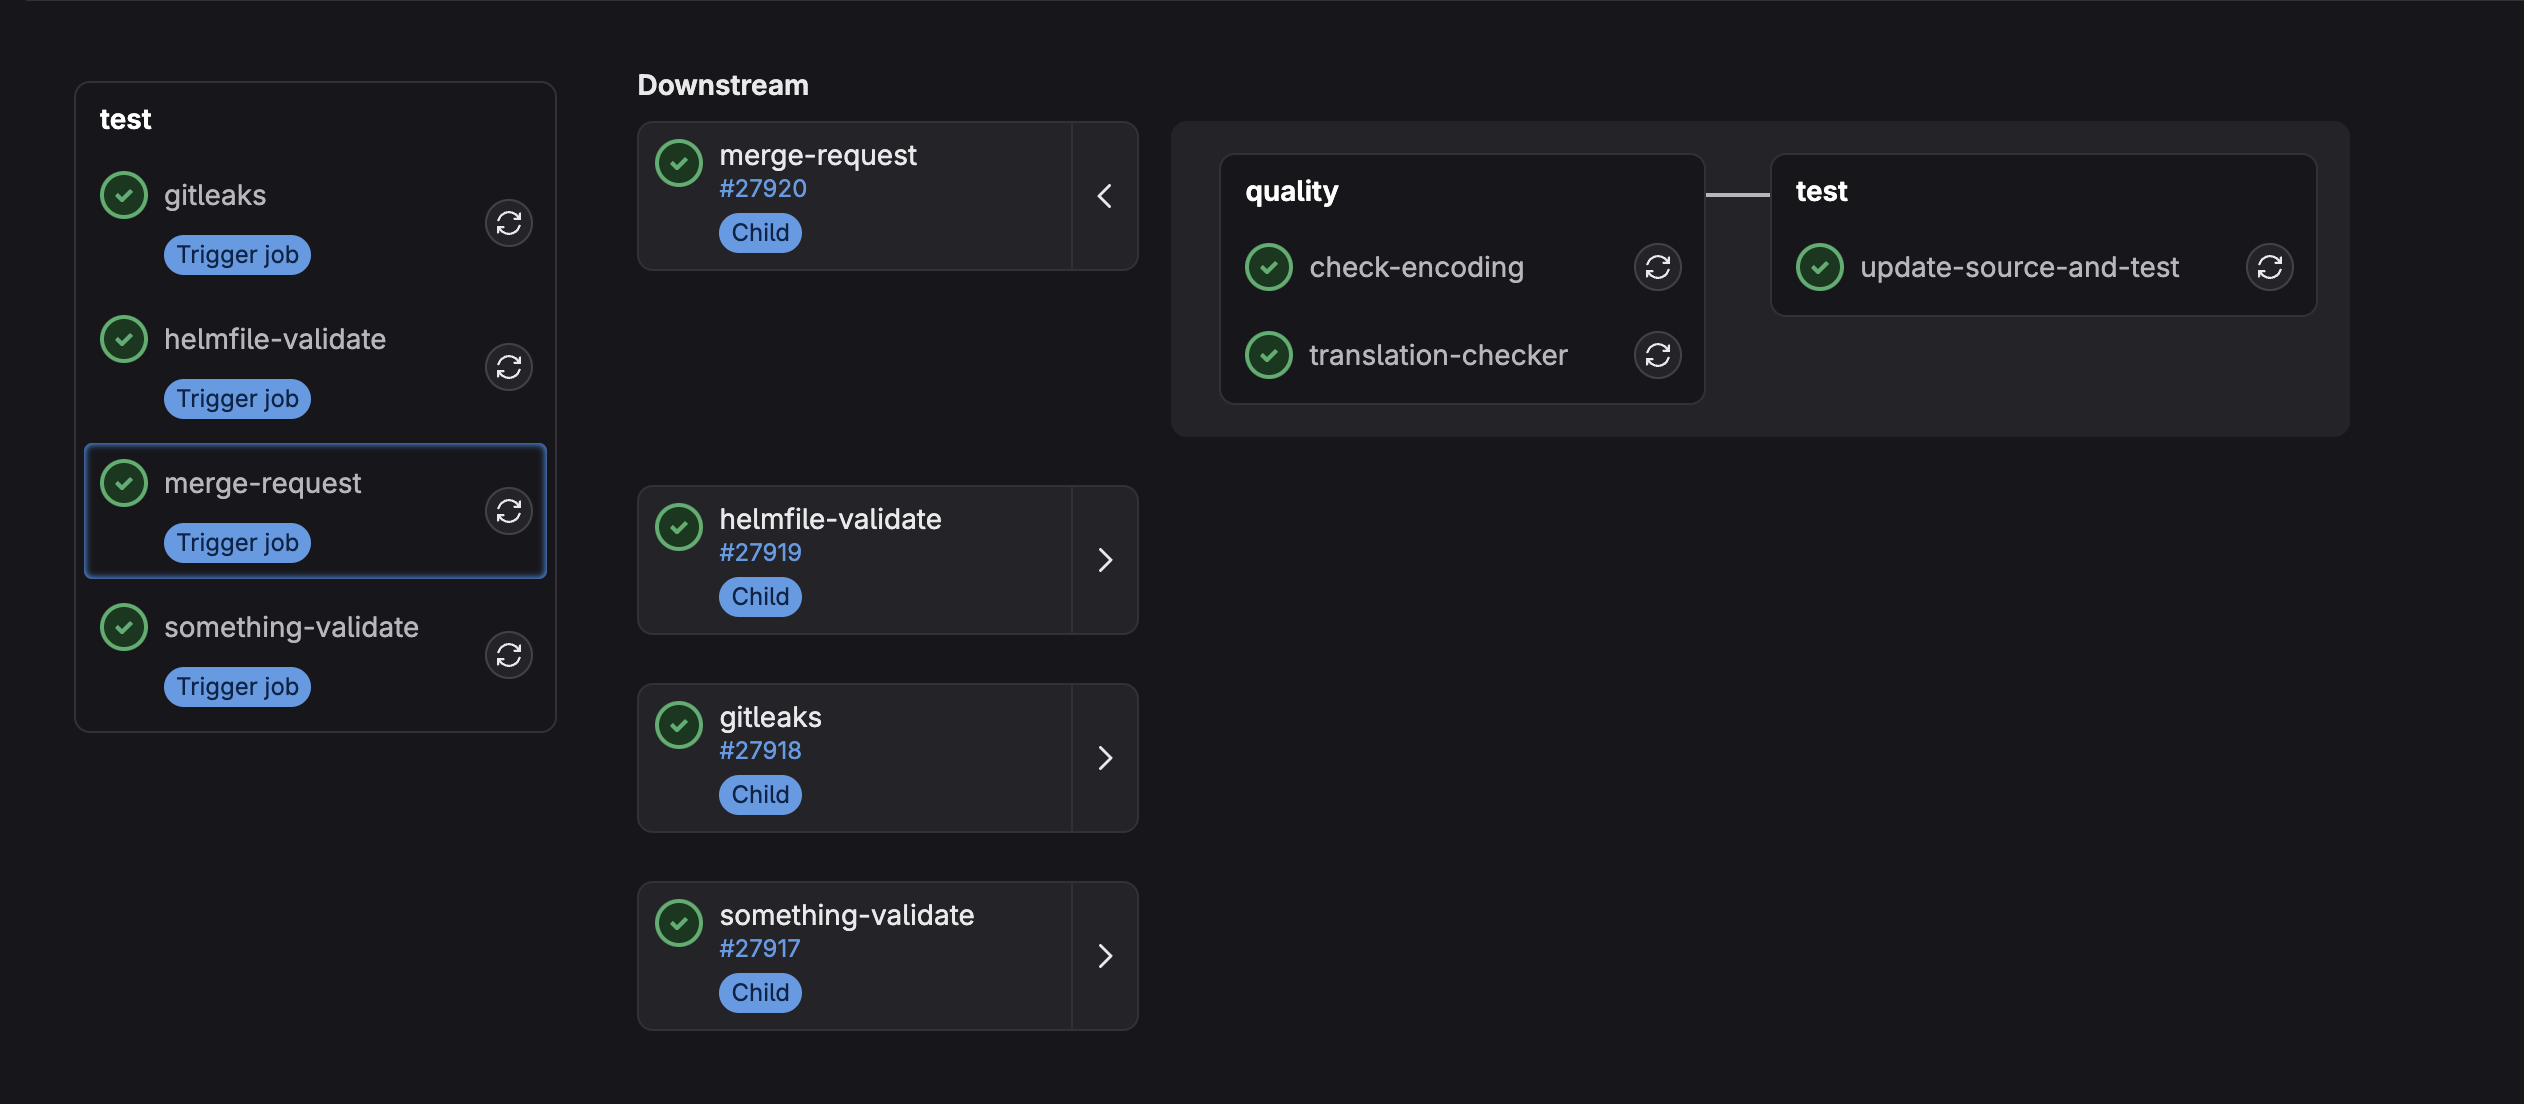
\includegraphics[width=16cm]{img/pipeline-run-result}
  \caption{Результат работы конвейера}
  \label{fig:pipeline-run-result}
\end{figure}

\section{Консольное приложение для автоматического переноса репозиториев из GitHub в GitLab} \label{sec:gitlab-migrator-app}
Консольное приложение, далее именуемое мигратором, представляет собой конечный автомат\cite{fsm} с возможностью запуска нескольких экземпляров одновременно.
Это необходимо, так как импорт репозитория в GitLab может занимать значительное время, и этот простой можно компенсировать параллельным запуском мигратора для нескольких репозиториев.
Архитектура приложения достаточно проста (Рис. \ref{fig:gitlab-migrator-app-architecture}), что соответствует его основной задаче: запускать определенный процессор, обрабатывать ошибки и фиксировать результаты работы.

\begin{figure}[H]
  \centering
  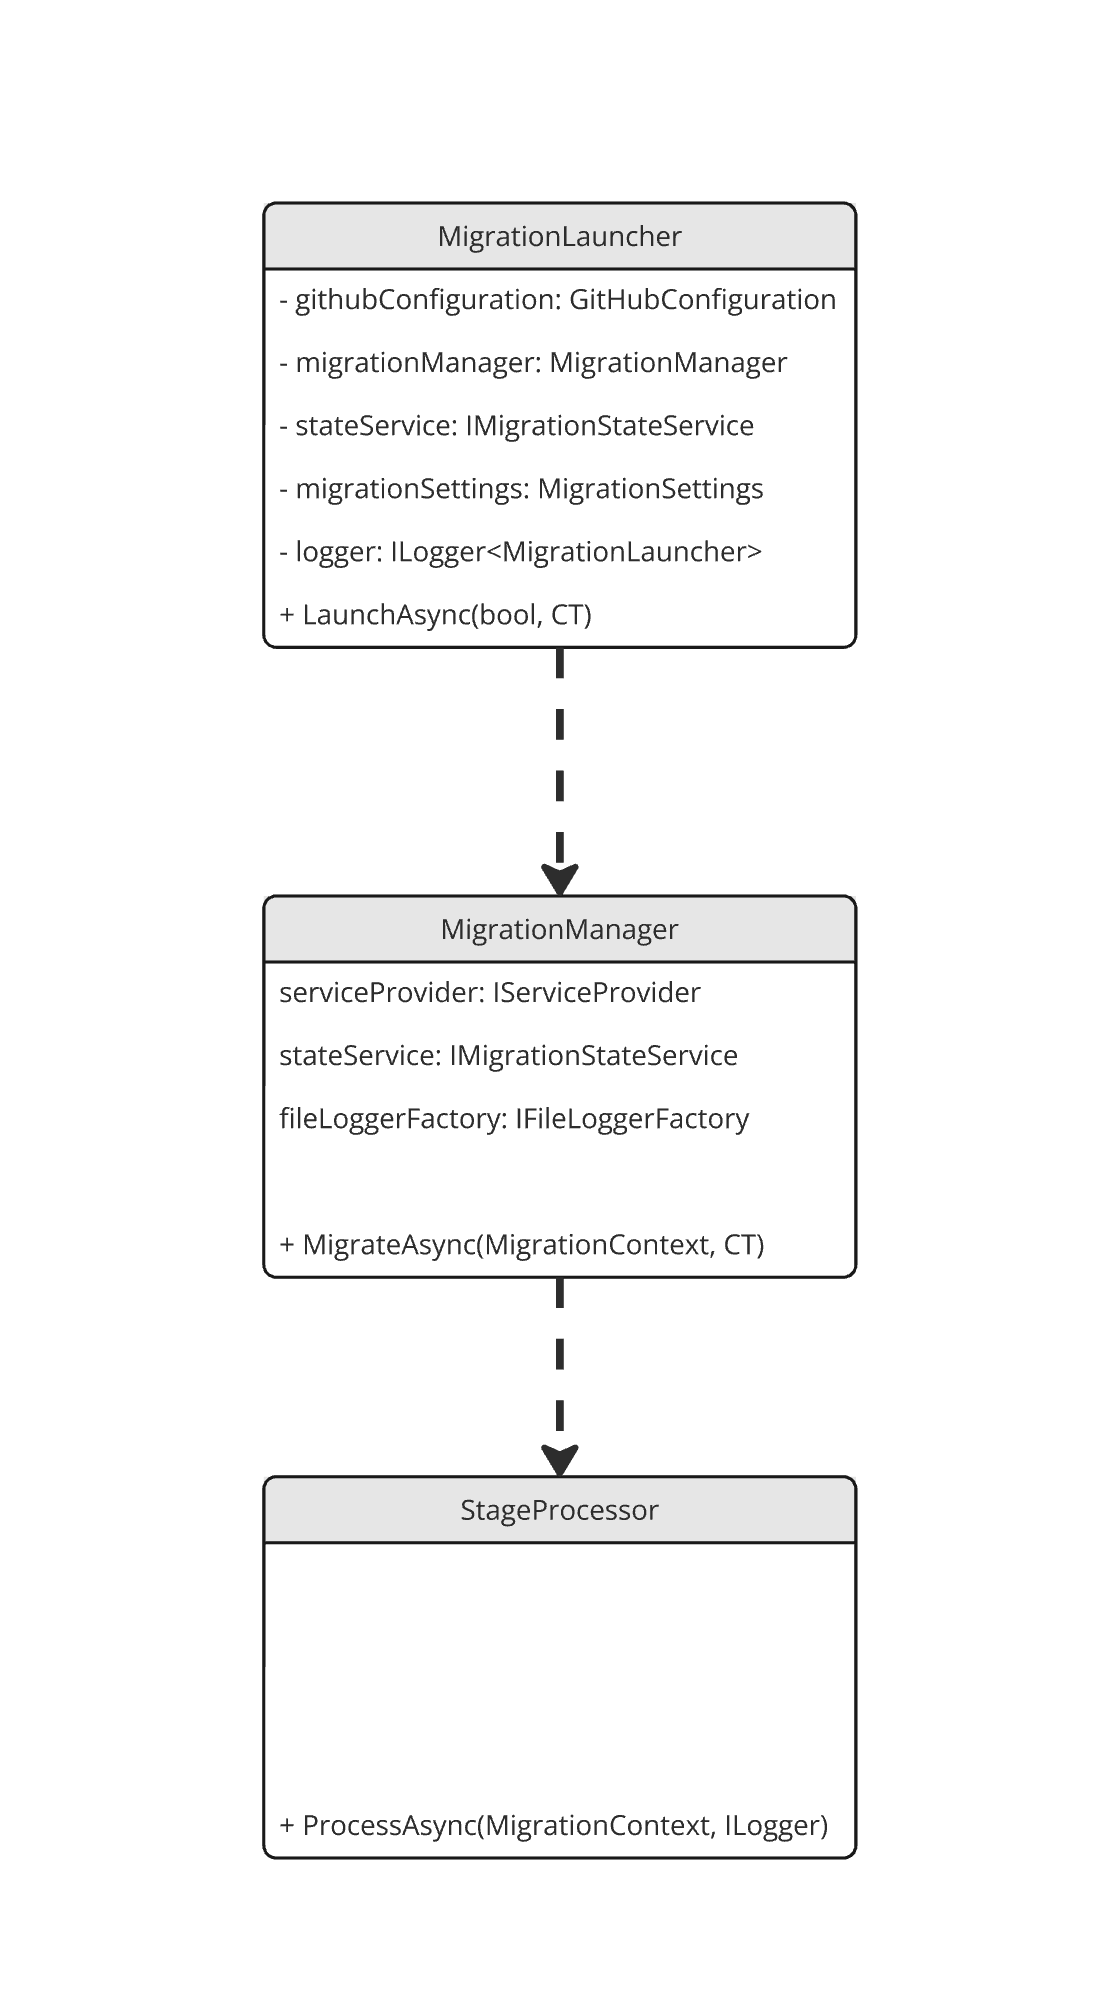
\includegraphics[width=10cm]{img/gitlab-migrator-app-architecture}
  \caption{Архитектура мигратора}
  \label{fig:gitlab-migrator-app-architecture}
\end{figure}

Поскольку пользователь может в любой момент завершить работу консольного приложения, необходимо локальное хранилище для сохранения состояния миграции.
Для этого был выбран YAML-файл: причина была в простоте и отсутствии необходимости более комплексных решений, например, отдельной базе данных.
Сам файл содержит всю необходимую информацию о репозиториях (Рис. \ref{fig:migration-state-file}).
Для создания и поддержания актуальности этого файла используется отдельная консольная команда,
которая взаимодействует с сетевым интерфейсом сервиса GitHub для получения данных о репозиториях и сетевым интерфейсом сервиса Google Sheets для получения информации о принадлежности репозитория определенной команде организации.
Актуализация данных происходит автоматически с помощью запланированной задачи, которая периодически запускает команду и фиксирует изменения в репозитории.

\begin{figure}[H]
  \centering
  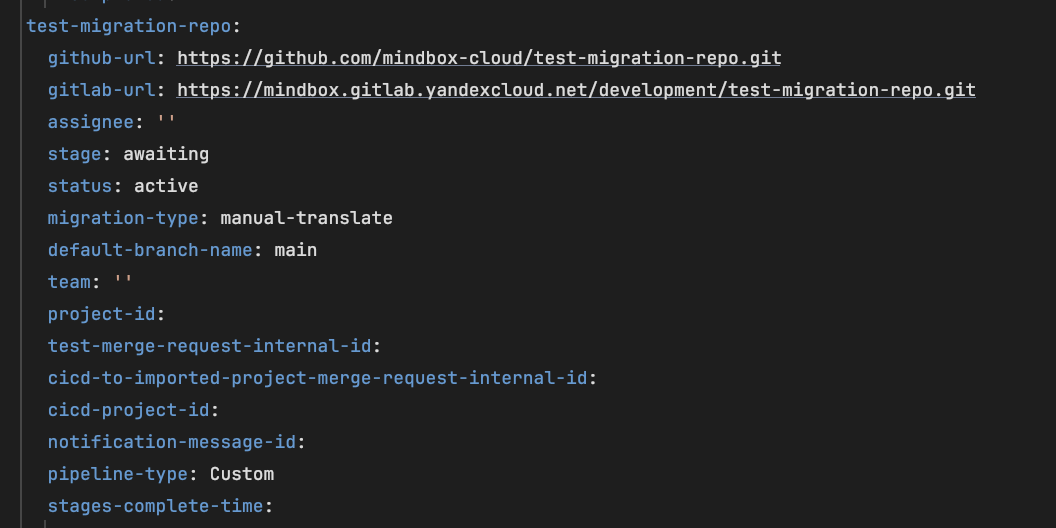
\includegraphics[width=12cm]{img/migration-state-file}
  \caption{Пример данных в YAML-файле для репозитория}
  \label{fig:migration-state-file}
\end{figure}

Принцип работы мигратора при переносе репозиториев следующий:
\begin{enumerate}
  \item \texttt{MigrationLauncher} выбирает репозитории, которые пользователь отметил для переноса (вписал свое имя в поле \texttt{assignee}).
  \item Далее этот класс запрашивает данные из общего YAML-файла и создает соответствующее количество экземпляров \texttt{MigrationManager},
        каждый из которых отвечает за миграцию одного репозитория.
  \item \texttt{MigrationManager} с помощью \texttt{IServiceProvider} находит \texttt{IStageProcessor},
        соответствующий текущему этапу миграции, и запускает его.
  \item После выполнения этапа процессор возвращает следующий шаг или ошибку, которую необходимо обработать и записать.
\end{enumerate}

Для удобства работы с промежуточными записями работы программы была реализована обертка над \texttt{ILogger},
которая перенаправляет записи в отдельный файл.

Всего в миграторе 30 шагов.
Каждый шаг содержит идемпотентную логику, связанную с определенным аспектом переноса проекта с GitHub на GitLab.
Это полезно в случае, если работа мигратора прерывается на середине какого-либо шага, то при следующем запуске сторонние эффекты предыдущих запусков не будут накапливаться, и результат будет таким же, как если бы прерывания не было.
Таким образом несколько разработчиков, даже без глубокого знания GitLab и самого мигратора, могут быстро и качественно выполнять миграцию.
В связи с этим каждый шаг достаточно атомарен и обрабатывает небольшую логику.
При этом шаги реализованы как сервисы в единственном экземпляре, что позволяет использовать инъекцию зависимостей.

Шаги миграции разделены на три фазы:
\begin{enumerate}
  \item Фаза переноса конфигураций конвейера в GitLab;
  \item Проверка корректности конвейера на уровне запроса на слияние;
  \item Полноценный импорт репозитория из GitHub с его архивацией и последующим слиянием перенесенной конфигурации конвейера.
\end{enumerate}

Далее описаны общие шаги мигратора в каждой из фаз.

\section{Фаза портирования конвейера в GitLab и проверка корректности на уровне запроса на слияние} \label{sec:first-and-second-phases}
Изначально вторая фаза включала проверку корректности конвейера как на уровне запроса на слияние, так и на уровне создания новой версии сервиса.
Однако в текущей реализации проверка корректности конвейера выпуска (release) была перенесена в третью фазу, что сделало вторую фазу менее объемной.
Поэтому здесь она рассматривается совместно с первой фазой.

\begin{enumerate}
  \item Уведомление в мессенджер о начале портирования конвейера репозитория.
        Канал отправки зависит от указанной команды;
  \item Локальное клонирование репозитория с префиксом \texttt{*cicd} и создание ветки для тестирования;
  \item Замена источника пакетов NuGet\cite{nuget} на GitLab в файле конфигурации и всех упоминаний GitHub в YAML и Docker файлах;
  \item Опциональная трансляция \emph{скелета} конвейера.
        Выполняется только при выборе определенного \texttt{MigrationType};
  \item Отображение подсказок в консоли, зависящих от типа репозитория.
        Например, для библиотек может быть предложено увеличить минорную версию, а для сервисов — заменить старое хранилище образов.
        Подсказки добавляются с помощью \texttt{KeyedSingleton}, что позволяет повторно использовать их в разных шагах без нарушения принципа избежаний дубликатов;
  \item Автоматическое создание запросов на слияния из ветки для тестирования в основную ветку.
        Проверяется результат выполнения конвейера.
        Ожидание завершения конвейера реализовано через возвращение шагом самого себя, что позволяет мигратору периодически проверять статус;
  \item При падении конвейера мигратор возвращается к шагу \texttt{merge\_request\_pipeline\_changes\_required}, чтобы пользователь мог исправить ошибки и повторить проверку.
        Для этого необходимо внести изменения в ветку для тестирования и перезапустить мигратор.
        Шаги с таким поведением помечены специальным атрибутом, что позволяет \texttt{MigrationManager} завершить работу при переходе на такой шаг.
\end{enumerate}

\section{Полноценный импорт репозитория из GitHub с архивацией и слиянием перенесенной конфигурации конвейера} \label{sec:third-phase}

\begin{enumerate}
  \item Уведомление в мессенджер о начале импорта репозитория, а в конце работы и о завершении миграции.
        Канал отправки зависит от указанной команды;
  \item Архивирование репозитория в GitHub для предотвращения рассинхронизации с GitLab;
  \item Импорт репозитория из GitHub в GitLab и ожидание завершения процесса.
        Он выполняется с помощью ранеупомянутого встроенного инструмента GitLab;
  \item Шаг с подсказками, аналогичный предыдущему, но с другим набором рекомендаций;
  \item Автоматическое обновление настроек проекта в Octopus Deploy, включая изменение различных переменных шагов, например, источник получаемого кода на встроенный вариант вместо GitHub;
  \item Создание запроса на слияние в импортированном репозитории на основе ранее протестированной ветки.
        Поскольку конвейер уже был проверен, он сразу сливается с мигратором, и мигратор отслеживает результат выполнения конвейера выпуска или добавлений изменений в основную ветку;
  \item При неудачном выполнении конвейера изменения откатываются, и мигратор возвращается к шагу \texttt{release\_pipeline\_changes\_required}.
        Пользователь должен исправить ошибки в ветке для тестирования и перезапустить мигратор;
  \item Перенос настроек, которые не поддерживаются встроенным импортом: настройки репозитория, например: политики слияния, защищенные ветки и множества правил (rulesets), отсутствующие в GitLab и требующие ручного сопоставления с доступными настройками.
        Также выполняется настройка прав доступа для групп и отдельных пользователей.
  \item Разархивация репозитория в GitHub и переключение его в режим чтения для всех пользователей.
        Необходимо, так как в компании есть автоматизация, основанная на Terraform модуле, которому необходимо, чтобы репозиторий не был заархивирован.
\end{enumerate}

%% TODO: conclusion
